\section{Verwandte Arbeiten}

\begin{figure*}
    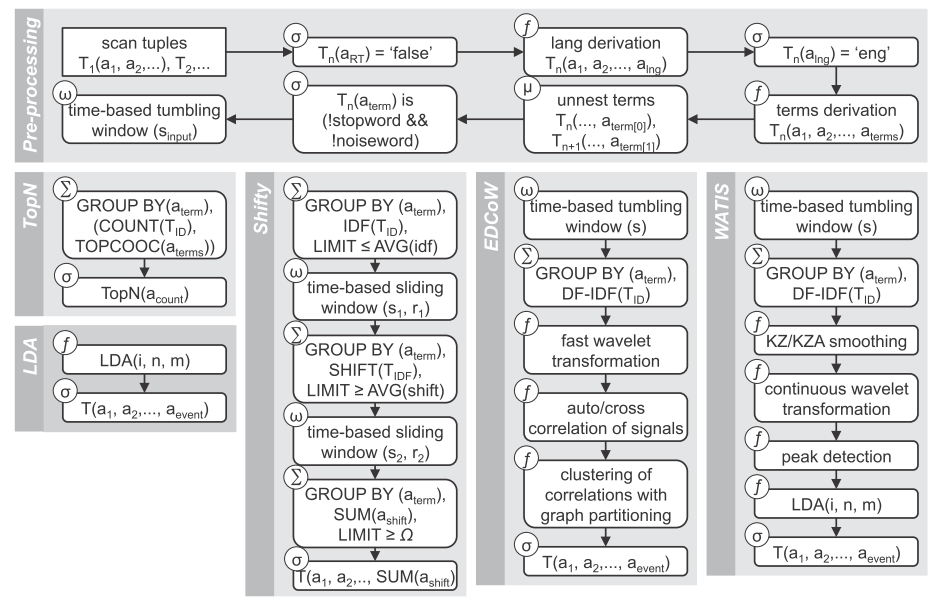
\includegraphics[width=\textwidth]{images/eventdetect.png}
    \caption{Niagarino Anfragen der fünf Erkennungs-Methoden}
    \label{fig:eventdetect}
\end{figure*}

\subsection{Event-Driven Detection}
Weiler et. al. \cite{weiler2016evaluation} evaluieren fünf State of the Art Techniken zur Erkennung von noch unbekannten Ereignissen.Niagarino wird als Implementation verwendet, eine Plattform die Apache Storm ähnelt. Die Techniken wurden als Anfragen umgesetzt, wie in \ref{fig:eventdetect} dargestellt.  Twitter-Events dienen als Datenbasis, die einem Pre-Processing gefiltert werden. Dabei werden Retweets entfernt und der Inhalt der restlichen Tweets gesäubert, es verbleiben bibliographisch erkannte englische Wörter. 

\begin{itemize}
\item TopN\\Jedem Wort wird ein Wert zugewiesen, der auf dem Inverse-Document-Frequency des Zeitfenster beruht. Nur die N-Wichtigtsten Wörter verbleiben als Event.
\item Latent Dirichlet Allocation (LDA)\\Ist ein hierarchisches Bayes-Modell, das die Variation des Vokabulars in einer Gruppe von Dokumenten bewertet. Für jedes Zeitfenster extrahiert LDA  vermutete Ereignisse, die durch Ausdrücke beschrieben werden. 
\item Shifty\\Dabei werden die Veränderungen von TopN bewertet die sich zwischen zwei Zeitfenstern ereignen.
\item Event Detection with Clustering of
Wavelet-based Signals (EDCoW)\\Der Stream wird Batches aufgeteilt, die dann per Wavelet-Analyse zu einem weiteren Event zusammengefasst werden, in dem Wörter mit erkannten Bursts stehen. Davon werden dann unwichtige Wörter entfernt. Durch Clustering erhält das Ergbnis Burst-Events die mit zwei Termen beschreiben werden.
\item The Wavelet Analysis Topic Inference Summarization
(WATIS)\\ Eine Weiterentwicklung des (EDCoW), bei dem zu jedem Burst fünf Terme geliefert werden.
\end{itemize}

\subsection{Burst Detection}
Da sich die Erkennung globaler Events mittels Esper als zumindest unvollständig erwies, wurden Methoden untersucht um das Verfahren zu Ergänzen oder zu Ersetzen.\\

Globale Events haben unter Anderem auch die Eigenschaft eine erhöhte Aktivität im Edit-Event-Stream zu verursachen. Erhöhte Aktivität (Bursts) ist ein Phänomen das bereits seit Jahrzehnten untersucht wird, daher existieren eine Reihe von Theorien und abgeleiteten Algorithmen. Dabei ist die zeitnahe Erstellung von Ergebnissen wichtig, weswegen auf eine wenig aufwändige Verarbeitung optimiert wird. Bursts besitzen eine Reihe an Attributen, die abhänig vom Use Case defininert werden. Dazu zählt der Zeitraum der jeweils auf das Auftreten eines Bursts untersucht wird, die Intensistät und die Verteilung der Intensistät auf den betrachteten Zeitraum.


Online Burst Detection Over High Speed Short Text Streams
\cite{yuan2007online}


Event Detection with Burst Information Networks
\cite{ge2016event}

Realtime
Die Realtime-Burst Detection über mehrere Fenstergrößen ist für die Analyse von Datenströmen hilfreich. Die üblichen Burst-Detektionsverfahren sind für die Echtzeiterkennung nicht effektiv. Die Realtime-Burst Detection benötigt eine neue Burst-Erkennungsmethode, die die Berechnung reduziert, indem redundante Datenaktualisierungen vermieden werden. Dabei wird ein Ereignis bei seinem Auftreten daraufhin analysiert inwiefern die Ankunftshäufigkeit und im Vergleich zur vorherigen Perioden ansteigt.

\cite{ebina2011real}
A real-time burst detection method

Efficient Elastic Burst Detection in Data Streams 
\cite{Zhu:2003:EEB:956750.956789}

Detecting ‘bursts’ in time series data with Kleinberg’s burst detection algorithm
\cite{kleinberg1}

\subsection{Social Media Analyse}

Wikipedia

Extracting Event-Related Information from
Article Updates in Wikipedia
\cite{10.1007978-3-642-36973-5_22}


\cite{gottschalk2017ongoing},
  Ongoing events in Wikipedia: a cross-lingual case study

\cite{fetahu2015much},
  How much is Wikipedia Lagging Behind News?

\cite{liu2016event}
  Event analysis in social multimedia: a survey

A cloud-enabled automatic disaster analysis system of multi-sourced data streams: An example synthesizing social media, remote sensing and Wikipedia data
\cite{huang2017cloud}

Pinterest
I need to try this?: a statistical overview of pinterest
\cite{gilbert2013need}

Twitter
An evaluation of the run-time and task-based performance of event detection techniques for Twitter
\cite{weiler2016evaluation}
